\documentclass{ximera}

\author{Anna Davis \and Paul Zachlin} \title{Isomorphic Vector Spaces} \license{CC-BY 4.0}

\renewcommand{\vec}[1]{{\bf #1}}
\newcommand{\RR}{\mathbb{R}}
\newcommand{\dfn}{\textit}
\newcommand{\dotp}{\cdot}

\newtheorem{general}{Generalization}
\newtheorem{initprob}{Exploration Problem}
\usepackage{tikz-cd}
\usepackage{tikz-3dplot}
\pgfplotsset{compat=1.14}



\begin{document}
\begin{abstract}
  We examine the effect of one-to-one and onto linear transformations on bases and other linearly independent and spanning sets.  We define isomorphic vector spaces and prove that any two vector spaces of the same finite dimension are isomorphic.
\end{abstract}
\maketitle



\section*{Some Results Concerning One-to-One Transformations and Onto Transformations}

Recall that a transformation $T$ is \dfn{one-to-one} provided that $$T(\vec{v}_1)=T(\vec{v}_2)$$ implies that $$\vec{v}_1=\vec{v}_2$$

 We will show that images of linearly independent vectors under one-to-one linear transformations are linearly independent.  

\begin{theorem}\label{th:onetoonelinind} Let $T:V\rightarrow W$ be a one-to-one linear transformation.  Suppose $\{\vec{v}_1,\ldots,\vec{v}_n\}$ is linearly independent in $V$.  Then $\{T(\vec{v}_1),\ldots,T(\vec{v}_n)\}$ is linearly independent in $W$.
\end{theorem}

\begin{proof}
Suppose $a_1, \ldots, a_n$ satisfy
\begin{align}\label{onlysolution}a_1T(\vec{v}_1)+\ldots +a_nT(\vec{v}_n)=\vec{0}\end{align}
We will show that for each $i$, we must have $a_i=0$.

By linearity, we have:
\begin{align*}\vec{0}&=a_1T(\vec{v}_1)+\ldots +a_nT(\vec{v}_n)\\
&=T(a_1\vec{v}_1)+\ldots +T(a_n\vec{v}_n)\\
&=T(a_1\vec{v}_1+\ldots +a_n\vec{v}_n)
\end{align*}
By Theorem \ref{th:zerotozero}, $T(\vec{0})=\vec{0}$.  Therefore,
$$T(a_1\vec{v}_1+\ldots +a_n\vec{v}_n)=T(\vec{0})$$

Because $T$ is one-to-one, we conclude that 
\begin{align}\label{onlytrivial}a_1\vec{v}_1+\ldots +a_n\vec{v}_n=\vec{0}\end{align}


By assumption, $\{\vec{v}_1,\ldots,\vec{v}_n\}$ is linearly independent.  Therefore $a_i=0$ for $1\leq i\leq n$.  
\end{proof}

Recall that a transformation $T$ is \dfn{onto} provided that every vector of the codomain of $T$ is the image of some vector in the domain of $T$.  

We will show that an onto linear transformation maps sets that span the domain to sets that span the codomain. 

\begin{theorem}\label{th:ontospan}
Let $T:V\rightarrow W$ be an onto linear transformation.  Suppose $V=\textnormal{span}(\vec{v}_1,\ldots ,\vec{v}_n)$.  Then $W=\textnormal{span}(T(\vec{v}_1),\ldots ,T(\vec{v}_n))$.
\end{theorem}
\begin{proof}
Suppose $\vec{w}$ is an element of $W$. To show that $\{T(\vec{v}_1),\ldots ,T(\vec{v}_n)\}$ spans $W$, we will express $\vec{w}$ as a linear combination of $T(\vec{v}_1),\ldots ,T(\vec{v}_n)$.

Because $T$ is onto, $\vec{w}=T(\vec{v})$ for some $\vec{v}$ in $V$.  But $V=\textnormal{span}(\vec{v}_1,\ldots ,\vec{v}_n)$.  Therefore, $\vec{v}=a_1\vec{v}_1+\ldots +a_n\vec{v}_n$ for some scalar coefficients $a_1,\ldots ,a_n$.
By linearity, we have:
\begin{align*}
\vec{w}=T(\vec{v})&=T(a_1\vec{v}_1+\ldots +a_n\vec{v}_n)\\
&=a_1T(\vec{v}_1)+\ldots +a_nT(\vec{v}_n)
\end{align*}
Thus, $\vec{w}$ is in the span of $T(\vec{v}_1),\ldots ,T(\vec{v}_n)$.
\end{proof}
 
Recall that a linear transformation that is one-to-one and onto is called an \dfn{isomorphism}.

We will now combine the results of Theorem \ref{th:onetoonelinind} and Theorem \ref{th:ontospan} to obtain a result about the effect of isomorphisms on a basis.

\begin{theorem}\label{th:bijectionsbasis}
Let $T:V\rightarrow W$ be an isomorphism.  Suppose $\mathcal{B}_V=\{\vec{v}_1,\ldots ,\vec{v}_n\}$ is a basis for $V$.  Then $\{T(\vec{v}_1),\ldots ,T(\vec{v}_n)\}$ is a basis for $W$.
\end{theorem}
\begin{proof}
Left to the reader.  (See Practice Problem \ref{prob:bijectionsbasisproof}) 
\end{proof}
 
 
%%%% Moved to Exercises %%%%%%%%%%%%%% 
%\begin{theorem} A linear transformation $T:V\rightarrow W$ is one-to-one if and only if $\text{ker}(T)=\{\vec{0}\}$.
%\end{theorem}
%\begin{proof}
%First assume that $T$ is one-to-one.  Suppose $\vec{v}$ is in $\text{ker}(T)$.  Then $T(\vec{v})=\vec{0}=T(\vec{0})$.  But then $\vec{v}=\vec{0}$.

%Next, assume that $\text{ker}(T)=\{\vec{0}\}$.  To show that $T$ is one-to-one, suppose $T(\vec{v}_1)=T(\vec{v}_2)$, but then
%\begin{align*}
%T(\vec{v}_1)-T(\vec{v}_2)&=\vec{0}\\
%T(\vec{v}_1-\vec{v}_2)&=\vec{0}
%\end{align*}
%Since the kernel only contains the zero vector, we conclude that
%$$\vec{v}_1-\vec{v}_2=\vec{0}$$
%Therefore
%$$\vec{v}_1=\vec{v}_2$$
%\end{proof}
 
\section{Isomorphic Vector Spaces}
\begin{definition} Let $V$ and $W$ be vector spaces.  If there exists an isomorphism from $V$ onto $W$ we say that $V$ and $W$ are isomorphic and write $V\cong W$.
\end{definition}

\begin{theorem}\label{th:ndimspacesisorn}
Let $V$ and $W$ be finite-dimensional vector spaces. Then
$$V\cong W\quad\text{if and only if}\quad \textnormal{dim}(V)=\textnormal{dim}(W)$$
\end{theorem}
\begin{proof}
First, assume that $V\cong W$.  Then there exists an isomorphism $T:V\rightarrow W$.  Suppose $\textnormal{dim}(V)=n$ and let $\{\vec{v}_1,\vec{v}_2,\ldots ,\vec{v}_n\}$ be a basis for $V$. By Theorem \ref{th:bijectionsbasis} $\{T(\vec{v}_1),\ldots ,T(\vec{v}_n)\}$ is a basis for $W$. Therefore $\textnormal{dim}(W)=n$.

Conversely, suppose $\textnormal{dim}(V)=\textnormal{dim}(W)=n$, and let $\mathcal{B}=\{\vec{v}_1,\vec{v}_2,\ldots ,\vec{v}_n\}$, $\mathcal{C}=\{\vec{w}_1,\vec{w}_2,\ldots ,\vec{w}_n\}$ be bases for $V$ and $W$, respectively.

Define a linear transformation $T:V\rightarrow W$ by $T(\vec{v}_i)=\vec{w}_i$ for $1\leq i\leq n$.  To show that $T$ is an isomorphism, we need to prove that $T$ is one-to-one and onto.

Suppose $T(\vec{u}_1)=T(\vec{u}_2)$ for some vectors $\vec{u}_1$, $\vec{u}_2$ in $V$.  We know that
$$\vec{u}_1=a_1\vec{v}_1+\ldots +a_n\vec{v}_n$$
$$\vec{u}_2=b_1\vec{v}_1+\ldots +b_n\vec{v}_n$$
for some scalars $a_i$'s and $b_i$'s.  Thus,
$$T(a_1\vec{v}_1+\ldots +a_n\vec{v}_n)=T(b_1\vec{v}_1+\ldots +b_n\vec{v}_n)$$
By linearity of $T$,
$$a_1\vec{w}_1+\ldots +a_n\vec{w}_n=b_1\vec{w}_1+\ldots +b_n\vec{w}_n$$
$$(a_1-b_1)\vec{w}_1+\ldots +(a_n-b_n)\vec{w}_n=\vec{0}$$
But $\vec{w}_1,\vec{w}_2,\ldots ,\vec{w}_n$ are linearly independent, so $a_i-b_i=0$ for all $1\leq i\leq n$.  Therefore $a_i=b_i$ for all $1\leq i\leq n$.  We conclude that $\vec{u}_1=\vec{u}_2$.

We now show that $T$ is onto. Suppose that $\vec{w}$ is an element of $W$.  Then $\vec{w}=c_1\vec{w}_1+\ldots +c_n\vec{w}_n$ for some scalars $c_i$'s.  But then
$$\vec{w}=c_1T(\vec{v}_1)+\ldots +c_nT(\vec{v}_n)=T(c_1\vec{v}_1+\ldots +c_n\vec{v}_n)$$
We conclude that $\vec{w}$ is an image of an element of $V$, so $T$ is onto.

\end{proof}

From this proof follows a corollary, that some would argue is a very important result.  It shows why we spent so much time trying to understand $\RR^n$ in this course!

\begin{corollary}\label{cor:ndimisotorn}
Every $n$-dimensional vector space is isomorphic to $\RR^n$.
\end{corollary}

\begin{example}
The span of any two linearly independent vectors in $\RR^3$ is isomorphic to $\RR^2$. %(See Figure \ref{fig:planeisoplane})


%\begin{figure}[h]
\begin{image}
\tdplotsetmaincoords{70}{130}
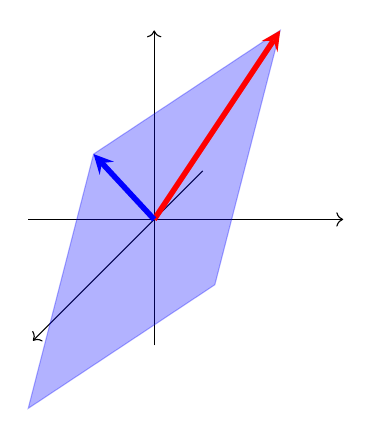
\begin{tikzpicture}[scale=0.8]
	\draw[->](-2,0,0)--(3,0,0) ;
    \draw[->](0,-2,0)--(0,3,0) ;
    \draw[->](0,0,-2)--(0,0,5) ;
    %\filldraw[blue, opacity=0.3] (0,0,0)--(4, 2, 0)--(5,6.5,5)--(0, 4, 5)--cycle;
   \filldraw[blue, opacity=0.3] (2,3,0)--(0,2,2.5)--(-2,-3,0)--(0,-2,-2.5)--cycle;
     
    
    \draw[->, line width=2pt,red, -stealth](0,0,0)--(2,3,0);
     \draw[->, line width=2pt,blue, -stealth](0,0,0)--(0,2,2.5);
    
\end{tikzpicture}~~~~~~~~~~~~~
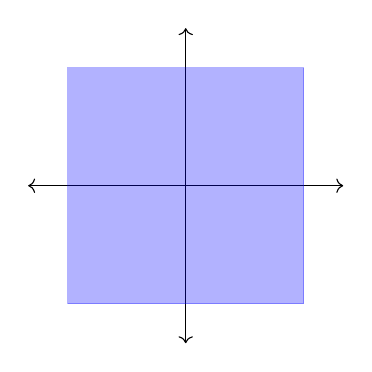
\begin{tikzpicture}[scale=0.5]

  \draw[<->] (-4,0)--(4,0);
  \draw[<->] (0,-4)--(0,4);
   \filldraw[blue, opacity=0.3] (-3,-3)--(-3,3)--(3,3)--(3,-3)--cycle;
 \end{tikzpicture}
%\caption{Two spaces of dimension 2 are isomorphic.}
  \label{fig:planeisoplane} 
  \end{image}
%\end{figure}

\end{example}

\begin{example}
The vector space $\mathbb{P}^2$ of polynomials of degree less than or equal to two from Example {\color{red} reference} is isomorphic to $\RR^3$.
\end{example}

\begin{explanation}
Recall that we defined $$\mathbb{P}^2=\left\{ax^2+bx+c : a,b,c \in \mathbb{R} \right\},$$ and we showed in Example {\color{red} reference} of module VSP-M-0060 that a basis for $\mathbb{P}^2$ is given by the three polynomials $\left\{1,x,x^2\right\}$.  Since $\textnormal{dim}\,\mathbb{P}^2=3=\textnormal{dim}\,\RR^3$, we conclude that $\mathbb{P}^2$ is isomorphic to $\RR^3$.
\end{explanation}
%Now I need to include this example in VSP-M-0060, which I probably would have anyways.

Isomorphisms are powerful tools that allow us to answer questions about unknown or inconvenient spaces using familiar or convenient spaces, such as $\RR^n$.  One such question is that of finding the matrix of a linear transformation for arbitrary vector spaces with arbitrary bases.  The following problem will pave the way to resolving this question. 

%{\color{green} Does this sound okay?}  YES!

\begin{initprob}\label{init:coordmapping} In this problem we will explore an isomorphism between an $n$-dimensional vector space and $\RR^n$.

Let $V$ be an $n$-dimensional vector space.  Then $V$ has a basis $\mathcal{B}=\{\vec{v}_1, \vec{v}_2,\ldots ,\vec{v}_n\}$.  Define a linear transformation $T:V\rightarrow \RR^n$ by $T(\vec{v}_i)=\vec{e}_i$ for $1\leq i\leq n$.
It is instructive to examine the action of $T$ on an arbitrary element of $V$.  Let $\vec{v}$ be an element of $V$, then $\vec{v}$ can be uniquely expressed as a linear combination of elements of $\mathcal{B}$.
$$\vec{v}=a_1\vec{v}_1+a_2\vec{v}_2+\ldots +a_n\vec{v}_n$$
By linearity we have
\begin{align*}
T(\vec{v})&=T(a_1\vec{v}_1+a_2\vec{v}_2+\ldots +a_n\vec{v}_n)\\
&=a_1T(\vec{v}_1)+a_2T(\vec{v}_2)+\ldots +a_nT(\vec{v}_n)\\
&=a_1\vec{e}_1+a_2\vec{e}_2+\ldots +a_n\vec{e}_n
\end{align*}
We can write this as $$T(\vec{v})=\begin{bmatrix}a_1\\a_2\\\vdots\\a_n\end{bmatrix}$$
Note that the components of $T(\vec{v})$ are the coefficients in front of the basis vectors in the linear combination that represents $\vec{v}$ in therms of the basis elements.  These coefficients are called \dfn{coordinates of $\vec{v}$ with respect to $\mathcal{B}$}.  The vector $T(\vec{v})$  is called the \dfn{coordinate vector of $\vec{v}$ with respect to $\mathcal{B}$}. We use the following notation to denote it

$$T(\vec{v})=\begin{bmatrix}a_1\\a_2\\\vdots\\a_n\end{bmatrix}=[\vec{v}]_{\mathcal{B}}$$

We leave it to the reader to verify that $T$ is an isomorphism.

\end{initprob}



\section*{Practice Problems}

\begin{problem}\label{prob:bijectionsbasisproof}
Prove Theorem \ref{th:bijectionsbasis}.
\end{problem}



\begin{problem}\label{prob:coordvector}
Let $V$ be a subspace of $\RR^3$ with a basis $\mathcal{B}=\left\{\begin{bmatrix}2\\1\\-1\end{bmatrix}, \begin{bmatrix}0\\3\\2\end{bmatrix}\right\}$.  Find the coordinate vector, $[\vec{v}]_{\mathcal{B}}$, for $\vec{v}=\begin{bmatrix}4\\-1\\-4\end{bmatrix}$.
$$[\vec{v}]_{\mathcal{B}}=\begin{bmatrix}\answer{2}\\\answer{-1}\end{bmatrix}$$
\end{problem}

\begin{problem}
If the order of the basis elements in Problem \ref{prob:coordvector} was switched to form a new basis
$$\mathcal{B}'=\left\{\begin{bmatrix}0\\3\\2\end{bmatrix}, \begin{bmatrix}2\\1\\-1\end{bmatrix} \right\}$$
How would this affect the coordinate vector?

$$[\vec{v}]_{\mathcal{B}'}=\begin{bmatrix}\answer{-1}\\\answer{2}\end{bmatrix}$$
\end{problem}

\begin{problem}\label{prob:verifyisomorphism}
Verify that $T:V\rightarrow \RR^n$ of Exploration Problem \ref{init:coordmapping} is an isomorphism.
\begin{hint}
You may find the proof of Theorem \ref{th:ndimspacesisorn} helpful.
\end{hint}
\end{problem}

\begin{problem} 
Prove that a linear transformation $T:V\rightarrow W$ is one-to-one if and only if $\text{ker}(T)=\{\vec{0}\}$.
\end{problem}


\end{document}
